\documentclass[a4,12pt]{report}

\usepackage[french]{babel}
\usepackage[utf8]{inputenc}
\usepackage[T1]{fontenc}
\usepackage{graphicx}
\usepackage{subcaption}
\usepackage{cleveref}
\usepackage[section]{placeins}
% Title Page
\title{ Rapport - TP IMA208}
\author{Renata PORCIUNCULA BAPTISTA}


\begin{document}
\maketitle
\section*{Introduction}
L'objective de ce rapport est présenter des résultats et conclusions des implémentations d'algorithme de traitement géométrique 3D en différents scenários de bruit et noyau. Les méthodes visent sont HPSS et APSS.

\section*{Partie I - HPSS}
\subsection*{1- L'ensemble aléatoire}
Nous avons utilisé $N=20000$, où $N$ est le numéro de points. Les images \ref{fig:1}, 2, 3 et 4 montrent les résultats pour le méthode HPSS. Ici, nous avons utilisé un poids directement proportionnel au distance carré. Nous avons noté le numéro de plus proche voisins $knn$ (en anglais, \textit{k-nearest neighbor}).

\begin{figure}[!h]
	\centering
	\begin{subfigure}[b]{0.5\textwidth}
		\centering
		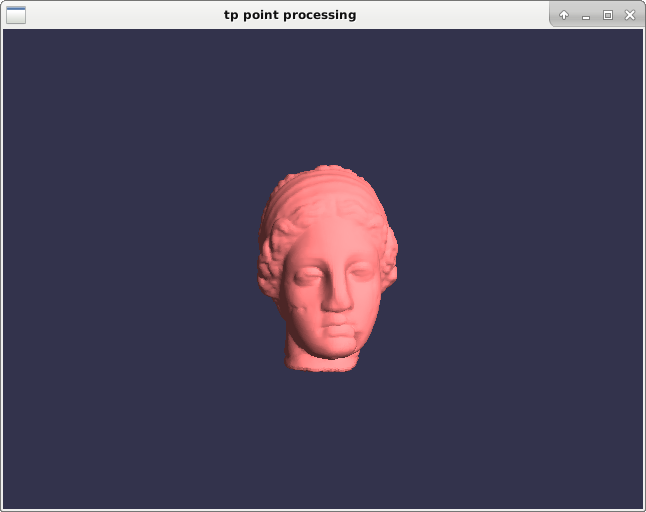
\includegraphics[height=1.8in]{figs/caso1-knn20-frontal-sem.png}
		\caption{Vision frontal}
	\end{subfigure}%
	\begin{subfigure}[b]{0.5\textwidth}
		\centering
		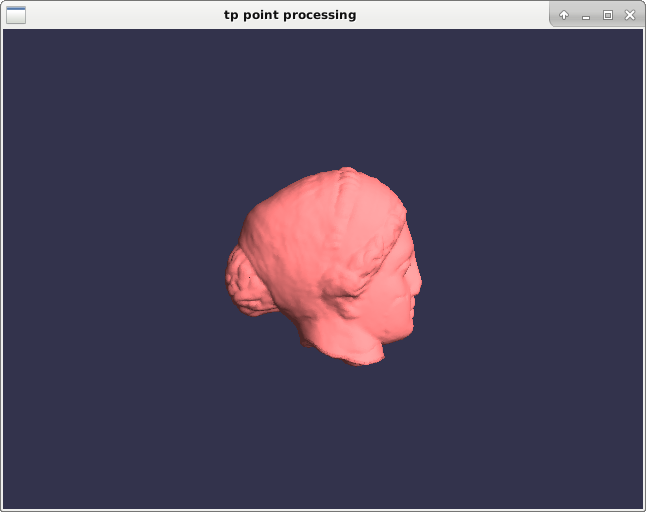
\includegraphics[height=1.8in]{figs/caso1-knn20-lateral-sem.png}
		\caption{Vision latéral}
	\end{subfigure}
	\caption{Résultat HPSS, $knn=20$, sans modèle.}
	\label{fig:1}
\end{figure}
\nopagebreak[4]
\begin{figure}[!h]
	\centering
	\begin{subfigure}[b]{0.5\textwidth}
		\centering
		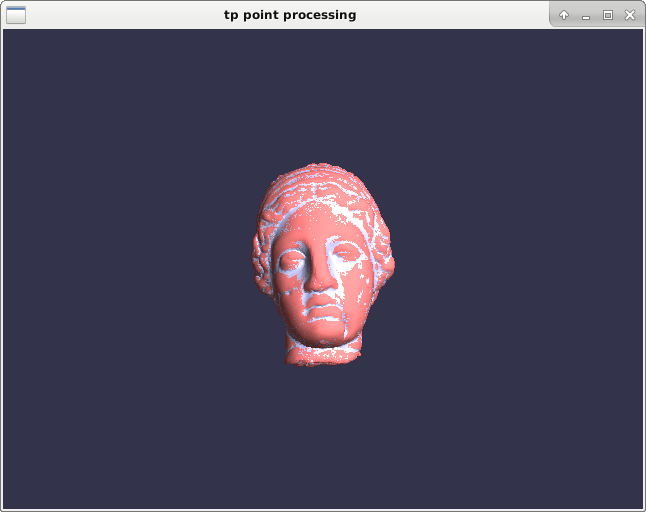
\includegraphics[height=1.8in]{figs/caso1-knn20-frontal-com.png}
		\caption{Vision frontal}
	\end{subfigure}%
	\begin{subfigure}[b]{0.5\textwidth}
		\centering
		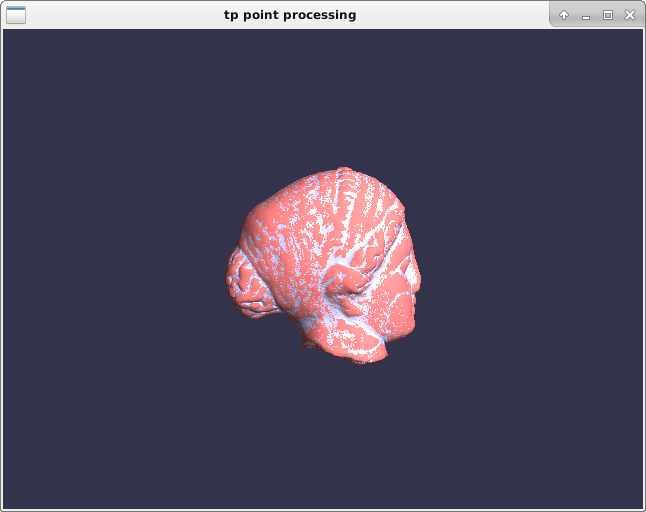
\includegraphics[height=1.8in]{figs/caso1-knn20-lateral-com.png}
		\caption{Vision latéral}
	\end{subfigure}
	\label{fig:2}
	\caption{Résultat HPSS, $knn=20$, avec le modèle.}
\end{figure}


\begin{figure}[!h]
	\centering
	\begin{subfigure}[b]{0.5\textwidth}
		\centering
		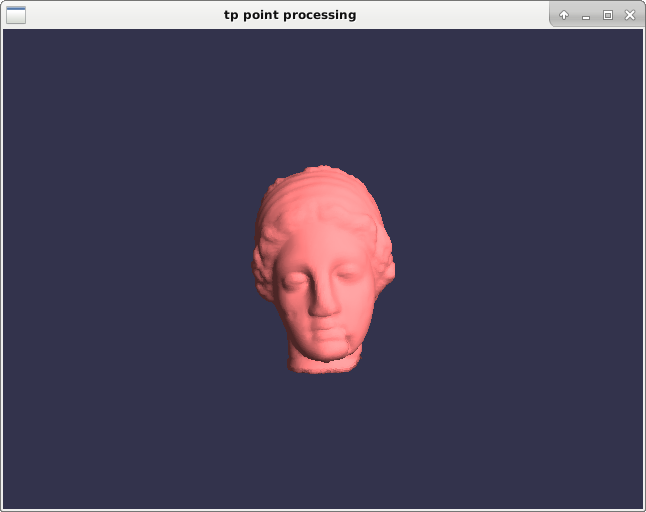
\includegraphics[height=1.8in]{figs/caso5-knn20-frontal-sem.png}
		\caption{Vision frontal}
	\end{subfigure}%
	\begin{subfigure}[b]{0.5\textwidth}
		\centering
		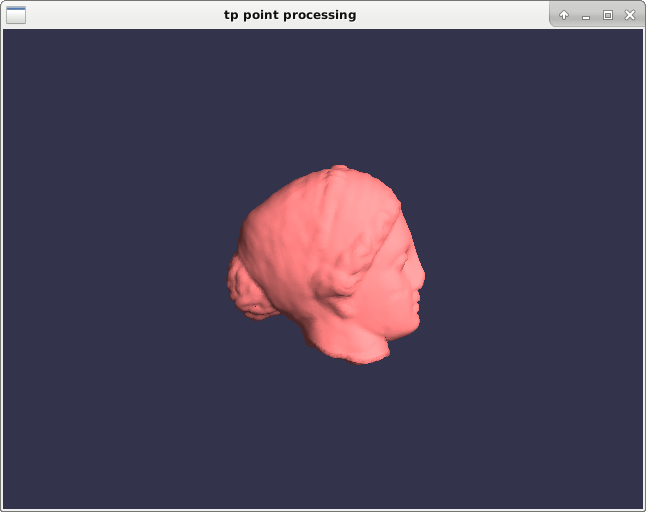
\includegraphics[height=1.8in]{figs/caso5-knn20-lateral-sem.png}
		\caption{Vision latéral}
	\end{subfigure}
	\caption{Résultat HPSS, $knn=40$, sans modèle.}
	\label{fig:9}
\end{figure}

\begin{figure}[!h]
	\centering
	\begin{subfigure}[b]{0.5\textwidth}
		\centering
		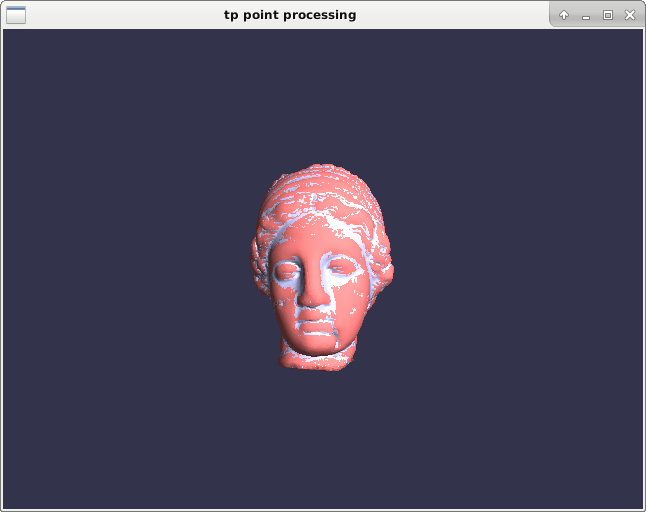
\includegraphics[height=1.8in]{figs/caso5-knn20-frontal-com.png}
		\caption{Vision frontal}
	\end{subfigure}%
	\begin{subfigure}[b]{0.5\textwidth}
		\centering
		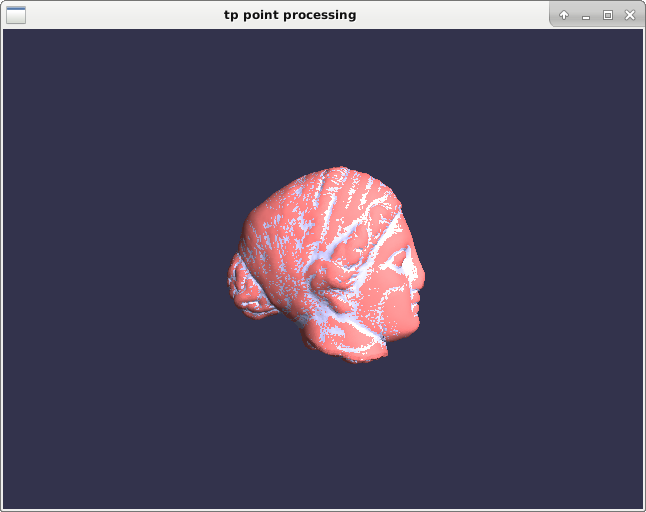
\includegraphics[height=1.8in]{figs/caso5-knn20-lateral-com.png}
		\caption{Vision latéral}
	\end{subfigure}
	\label{fig:10}
	\caption{Résultat HPSS, $knn=40$, avec le modèle.}
\end{figure}

Nous avons pu observer que le plus grand $knn$, plus lisse est le résultat. 

\pagebreak[4]
\subsection*{2- Noyau gaussien}

Nous avons utilisé $N=20000$, où $N$ est le numéro de points. Les images \ref{fig:3}, 6 montrent les résultats pour le méthode HPSS avec un noyau gaussien de différent radius. Dans ce scenário, $knn=20$.


\begin{figure}[!h]
	\centering
	\begin{subfigure}[b]{0.5\textwidth}
		\centering
		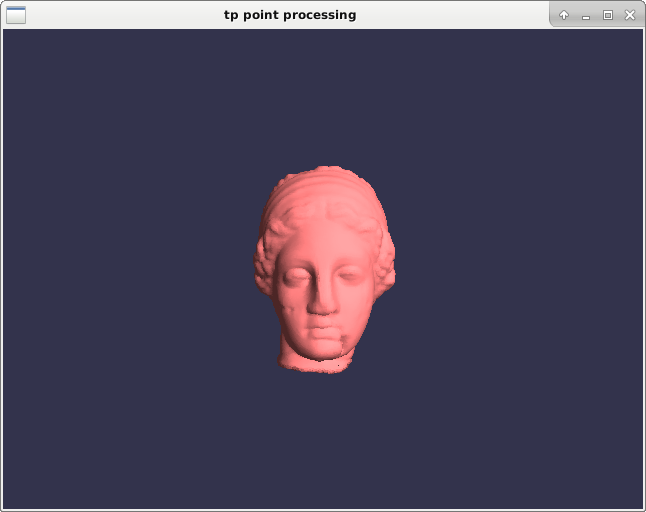
\includegraphics[height=1.8in]{figs/caso2-knn20-frontal-sem.png}
		\caption{Vision frontal}
	\end{subfigure}%
	\begin{subfigure}[b]{0.5\textwidth}
		\centering
		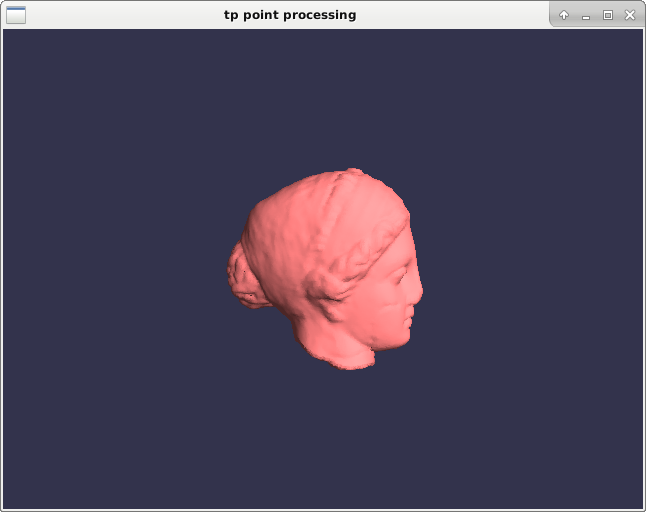
\includegraphics[height=1.8in]{figs/caso2-knn20-lateral-sem.png}
		\caption{Vision latéral}
	\end{subfigure}
	\caption{Résultat HPSS, $r=0.2$,  sans modèle.}
	\label{fig:3}
\end{figure}
\begin{figure}[!h]
	\centering
	\begin{subfigure}[b]{0.5\textwidth}
		\centering
		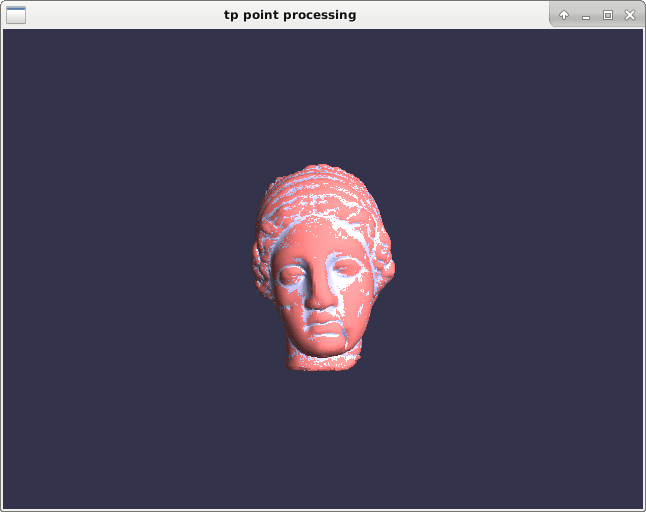
\includegraphics[height=1.8in]{figs/caso2-knn20-frontal-com.png}
		\caption{Vision frontal}
	\end{subfigure}%
	\begin{subfigure}[b]{0.5\textwidth}
		\centering
		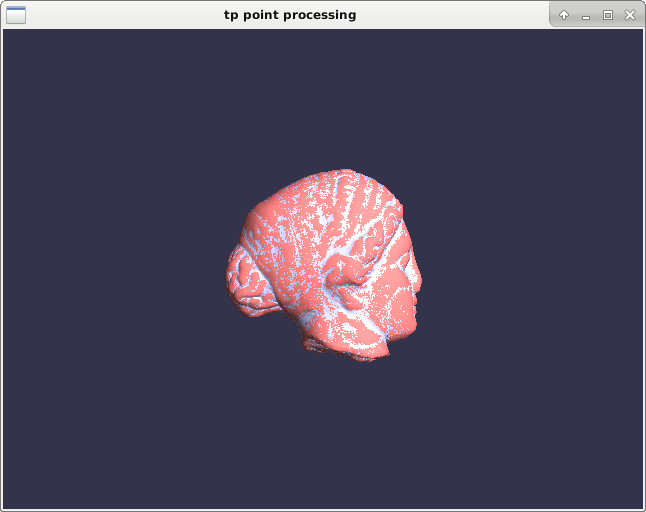
\includegraphics[height=1.8in]{figs/caso2-knn20-lateral-com.png}
		\caption{Vision latéral}
	\end{subfigure}
	\label{fig:4}
	\caption{Résultat HPSS, $r=0.2$, avec le modèle.}
\end{figure}


\begin{figure}[!h]
	\centering
	\begin{subfigure}[b]{0.5\textwidth}
		\centering
		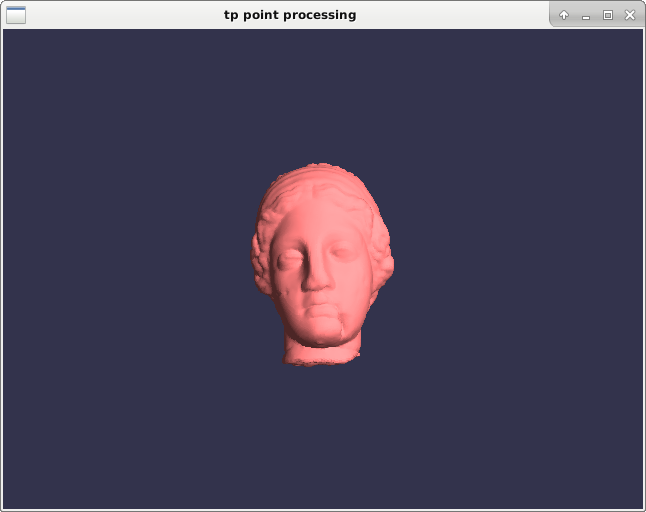
\includegraphics[height=1.8in]{figs/caso3-knn20-frontal-sem.png}
		\caption{Vision frontal}
	\end{subfigure}%
	\begin{subfigure}[b]{0.5\textwidth}
		\centering
		\includegraphics[height=1.8in]{figs/caso3-knn20-lateral-sem.png}
		\caption{Vision latéral}
	\end{subfigure}
	\caption{Résultat HPSS, $r=0.05$,  sans modèle.}
	\label{fig:5}
\end{figure}
\begin{figure}[!h]
	\centering
	\begin{subfigure}[b]{0.5\textwidth}
		\centering
		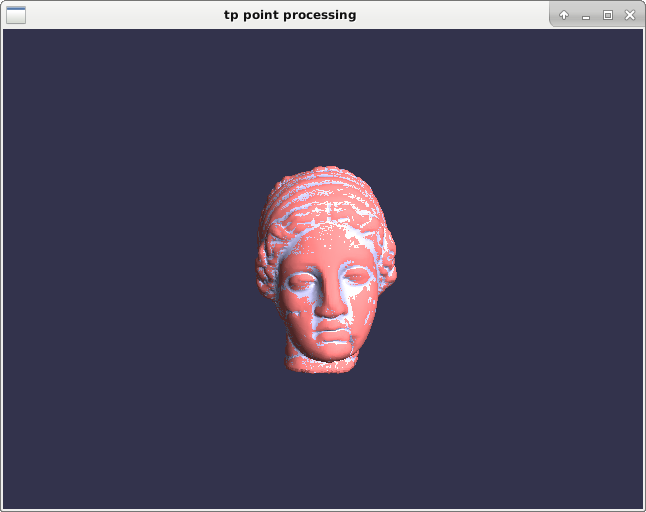
\includegraphics[height=1.8in]{figs/caso3-knn20-frontal-com.png}
		\caption{Vision frontal}
	\end{subfigure}%
	\begin{subfigure}[b]{0.5\textwidth}
		\centering
		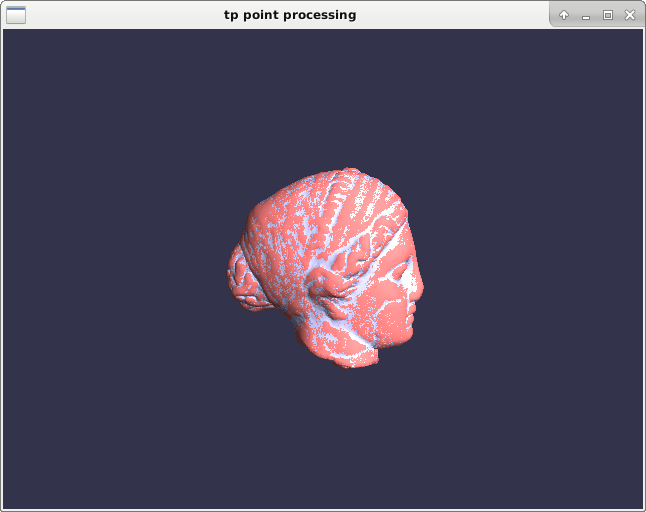
\includegraphics[height=1.8in]{figs/caso3-knn20-lateral-com.png}
		\caption{Vision latéral}
	\end{subfigure}
	\label{fig:6}
	\caption{Résultat HPSS, $r=0.05$, avec le modèle.}
\end{figure}

Nous avons peut observer qu'il y a une grand convergence de points dans les régions lisses. C'est résultat est dû le fonction de poids gaussien, qui marche comme um filtre de fréquences plus hautes. Donc, dans les fréquences plus bas, nous avons presque les mêmes points et dans les régions, dans lesquels il y a plus de variations, on a une courbure plus lisse que le modèle original.


Le plus grand le rayon de filtrage, plus de points sont utilisés pour définir la projection. Plus robuste.
Le plus plut petit le rayon de filtrage, moins de points utilisés pour définir la projection. 

Aussi, par rapport le poids de distances carrés, on a des meilleurs résultats.

\subsection*{3- Noyau gaussien avec le bruit}
Nous avons utilisé $N=20000$, où $N$ est le numéro de points. Les images \ref{fig:7} et \ref{fig:8} montrent les résultats pour le méthode HPSS avec un différents intensités de bruits. Dans ce scenário, $knn=20$, $r=0.2$.

\begin{figure}[!h]
	\centering
	\begin{subfigure}[b]{0.5\textwidth}
		\centering
		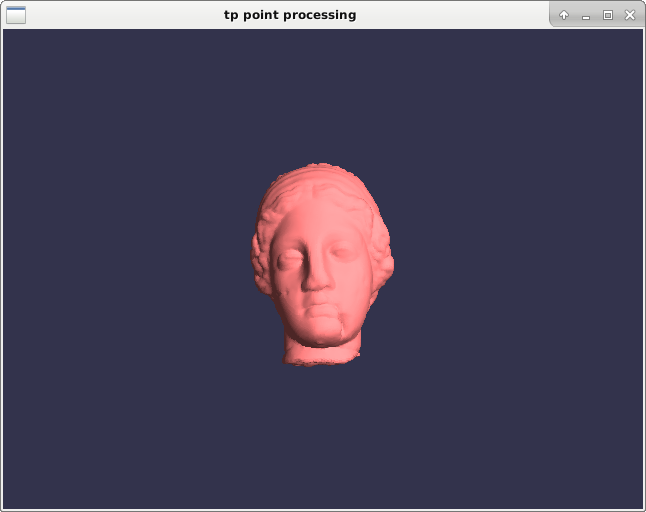
\includegraphics[height=1.8in]{figs/caso3-knn20-frontal-sem.png}
		\caption{Vision frontal}
	\end{subfigure}%
	\begin{subfigure}[b]{0.5\textwidth}
		\centering
		\includegraphics[height=1.8in]{figs/caso3-knn20-lateral-sem.png}
		\caption{Vision latéral}
	\end{subfigure}
	\caption{Résultat HPSS, bruit uniforme 0.5,  sans modèle.}
	\label{fig:7}
\end{figure}
\begin{figure}[]
	\centering
	\begin{subfigure}[b]{0.5\textwidth}
		\centering
		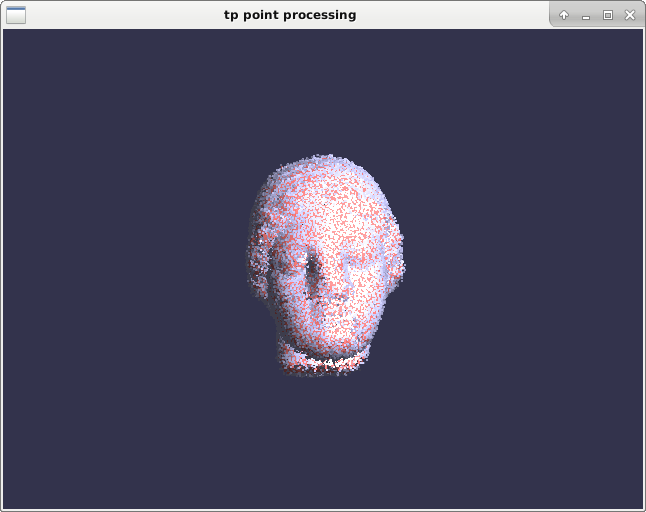
\includegraphics[height=1.8in]{figs/caso4-knn20-frontal-com.png}
		\caption{Vision frontal}
	\end{subfigure}%
	\begin{subfigure}[b]{0.5\textwidth}
		\centering
		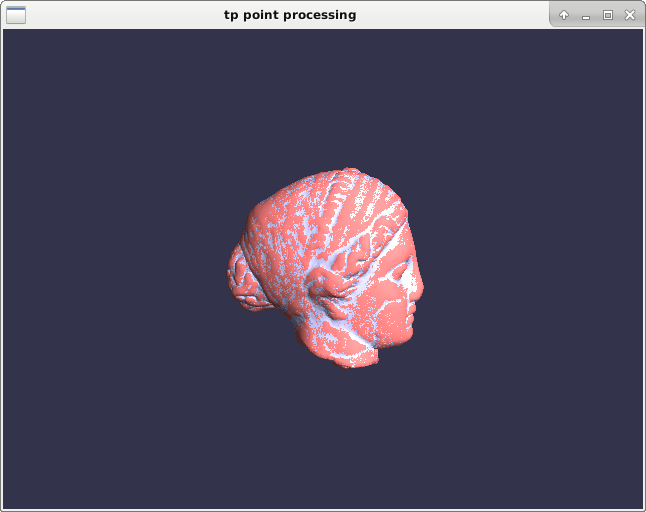
\includegraphics[height=1.8in]{figs/caso3-knn20-lateral-com.png}
		\caption{Vision latéral}
	\end{subfigure}
	\label{fig:8}
	\caption{Résultat HPSS, bruit uniforme 0.5, avec le modèle.}
\end{figure}
\pagebreak[4]
\section*{Part II - APSS}
\subsection*{1- APSS versus HPSS} 
Nous n'avons pas reussi à coder l'APSS.


\section*{Conclusion}
Nous avons réussi à implémenter l'algorithme HPSS et nous avons pu observer les influences de numéro de plus proches voisins, et du radius du noyau. Il y a un compris entre fidelité et bruit, c'est-á-dire, plus on filtre, moins de bruit, mais aussi on perd en texture et détails.
%\begin{abstract}
%\end{abstract}

\end{document}          
